\documentclass[preprint,12pt,nonatbib]{elsarticle}
\usepackage[T1]{fontenc}
\usepackage{amsmath,amssymb}
\usepackage{booktabs}
\usepackage{graphicx}
\usepackage{float}
\usepackage{xcolor}
\newcommand{\doiprefix}{https://doi.org/}
\usepackage[natbibapa]{apacite}
\shortcites{eckman2023,dumas2018,rozinat2009,camargo2020,chapela2023,chapela2025,rosenthal2021,knoll2019,rigas2018,lecuyer2002}
\usepackage[hidelinks]{hyperref}
\usepackage{xurl}
\newcommand{\VoneReps}{30}
\newcommand{\VoneCases}{100\,000}
\newcommand{\VoneWorst}{0.86\,\%}
\newcommand{\VoneCovered}{13 of 13}
\newcommand{\VoneLittle}{0.03\,\%}
\newcommand{\VtwoReps}{2}
\newcommand{\VtwoCases}{5\,000}
\newcommand{\VtwoBound}{262.0\,\%}
\newcommand{\VtwoZero}{13 of 13}
\newcommand{\VfourPartition}{1\times10^{-14}}
\newcommand{\VfourReps}{5}
\newcommand{\VfiveN}{2\,000}
\newcommand{\VfiveOfficeSingle}{26.3\,\%}
\newcommand{\VfiveOfficeKeyed}{19.8\,\%}
\newcommand{\VfiveOfficeIndep}{45.1\,\%}
\newcommand{\VfiveOfficeRep}{0.5\,\%}
\newcommand{\VfiveRatio}{19}
\newcommand{\VfiveWrong}{0.0\,\%}
\newcommand{\VfiveNs}{4.2\,\%}

\providecommand{\VsixMillion}{--}\providecommand{\VsixRate}{--}\providecommand{\VsixCpu}{--}\providecommand{\VsixNode}{--}\providecommand{\VsixChromium}{--}\providecommand{\VsixFirefox}{--}\providecommand{\VsixReps}{--}\providecommand{\VsixMismatches}{--}\providecommand{\VsixCompared}{--}\providecommand{\VsixMillionChromium}{--}\providecommand{\VsixMillionFirefox}{--}\providecommand{\VsixRatioMin}{--}\providecommand{\VsixRatioMax}{--}
\providecommand{\VthreeCases}{--}\providecommand{\VthreeLogCycle}{--}\providecommand{\VthreeOwnCycle}{--}\providecommand{\VthreeProCycle}{--}\providecommand{\VthreeDiff}{--}\providecommand{\VthreeApprox}{--}
\newcommand{\tool}{Process Simulator}
\journal{Simulation Modelling Practice and Theory}

\begin{document}
\begin{frontmatter}
\title{Process Simulator: an open, browser-based BPMN simulation environment with statistically controlled scenario comparison and simulation-based value stream mapping}
\author{Moritz Maier}
\affiliation{organization={Bern University of Applied Sciences (BFH)},city={Bern},country={Switzerland}}

\begin{abstract}
What-if analysis with business process simulation is usually done in tools that compare a single simulated run per scenario, and that report a value stream map only for straight sequences of steps. We present \tool, an open-source (Apache-2.0) discrete-event simulator for BPMN~2.0 that runs in the browser, as a Camunda Modeler plugin and as a command-line runner. It compares scenarios with replications, confidence intervals and common random numbers from per-source random streams, and derives value stream figures (lead time, process cycle efficiency, value-added and non-value-added time, rework and waiting) that also cover exclusive and parallel branches and loops. We verify the engine against exact queueing results (M/M/1, M/M/$c$, M/G/1, tandem and Jackson networks): all \VoneCovered{} confidence intervals cover the exact value, worst relative error \VoneWorst. A cross-check with Prosimos bounds the difference between the two engines to \VtwoBound; on a model discovered with Simod from the BPI Challenge 2012 log both engines agree within \VthreeDiff{} in mean cycle time. The value stream figures match closed-form results for sequences, choices, parallel splits and loops, where a linear map misstates process cycle efficiency. On a staffing problem, one run per scenario picks a wrong option in up to \VfiveOfficeIndep{} of the trials; ten paired replications reduce this to \VfiveOfficeRep. All results can be recomputed with one command.
\end{abstract}

\begin{keyword}
Business process simulation \sep BPMN \sep Discrete-event simulation \sep Common random numbers \sep Value stream mapping \sep Verification and validation \sep Open-source software
\end{keyword}
\end{frontmatter}

\section{Introduction}
\label{sec:intro}
A coffee-shop owner weighs three changes to her process: hiring a second barista, shifting the product mix to fifty-fifty, or both. She draws the process in BPMN, runs each option once in a simulation tool, and compares the reported mean cycle times. This is how wrong decisions are made: in the decision experiment of this paper, the option picked this way is wrong in up to \VfiveOfficeIndep{} of the trials (Section~\ref{sec:v5}), although nothing about the model differs between the runs; only the random numbers do.

Business process simulation (BPS) estimates the effect of changes such as additional staff, shorter activities or different routing before they are implemented \citep{vanderaalst2015,dumas2018}. Many BPM suites contain a simulator, and dedicated engines exist in research, notably BIMP (QBP) and Prosimos \citep{lopezpintado2022,lopezpintado2024}, together with tools that discover simulation models from event logs \citep{rozinat2009,camargo2020}. Surveys of tool support report heterogeneous and often limited simulation capabilities \citep{pereira2016,rosenthal2021,laue2016}.

Two practical gaps motivated the tool presented here. First, what-if results are commonly read from a single run per scenario. The statistical remedies, independent replications, confidence intervals and common random numbers (CRN), are textbook simulation methodology \citep{law2015,nelson1995,kim2001}, but they are rarely part of the modelling workflow of BPMN tools. Second, value stream mapping (VSM) \citep{rother1999} is widely used to discuss lead time and waste, and simulation-based VSM is established in manufacturing \citep{lian2007,solding2009}; process mining has been used to obtain value stream maps from logs \citep{knoll2019}. A value stream map, however, is designed around a sequence of steps, whereas BPMN models contain exclusive choices, parallel branches and loops; existing workarounds for parallel work are heuristic.

This paper describes \tool{} and, mainly, its verification. We do not claim that BPMN simulation, simulation-based VSM or the combination of a model editor with a simulator are new. Two technical contributions accompany the environment: a formally defined, trace-based partition of simulated case lead time into value stream categories that remains well defined under non-linear control flow (Section~\ref{sec:vsm}), and a per-source random-stream scheme that keeps common random numbers synchronised across structurally different scenarios (Section~\ref{sec:stats}). In full, the paper contributes:
\begin{enumerate}
\item modelling and simulation in one browser application without installation, and the same engine as a Camunda Modeler plugin and a command-line runner (Section~\ref{sec:tool});
\item scenario comparison with replications, Student-$t$ confidence intervals and paired differences under CRN, where each source of randomness has its own stream so that changing one activity does not shift the random numbers of the others (Section~\ref{sec:stats});
\item value stream figures computed from the simulated time line of each case, which partition lead time also for choices, parallel branches and loops (Section~\ref{sec:vsm});
\item an automated evaluation: exact queueing results, a cross-check with Prosimos, a model discovered from a public event log, closed-form VSM cases, decision quality of single runs versus replications, and run time (Section~\ref{sec:eval});
\item a reproducibility package under Apache-2.0 that recomputes every number in this paper with one command.
\end{enumerate}

\section{Related work}
\label{sec:related}
\paragraph{BPS tools and engines} BPS has a long tradition \citep{vanderaalst2015}; the BPSim standard defines simulation parameters for BPMN models \citep{laue2016}. \citet{pereira2016} and \citet{rosenthal2021} compare simulation support in BPM tools and observe large differences in the supported parameters and outputs. Prosimos is an open-source Python engine with differentiated resources, i.e.\ individual calendars and performance per resource \citep{lopezpintado2022}; it is the engine behind Simod, which discovers simulation models from event logs \citep{camargo2020,lopezpintado2024}. Our engine is simpler in this respect: resources form roles with a shared calendar and a single duration distribution per activity.

\paragraph{Quality of simulation models} Discovered models are usually assessed by comparing simulated and real logs \citep{chapela2023,chapela2025} or by their usefulness for downstream tasks \citep{oezdemir2025}. \citet{bluemel2026} show that data-preparation choices can change what-if conclusions on a real log. These works concern model discovery; we use a discovered model only to check that our engine reproduces a second engine on realistic input (Section~\ref{sec:v3}).

\paragraph{Comparing alternatives} Selecting the best of several simulated systems is the subject of ranking and selection \citep{bechhofer1954,kim2001}; CRN reduce the variance of differences between systems \citep{nelson1995,law2015}. Independent streams per source are a standard way to keep random numbers synchronised across scenarios \citep{lecuyer2002}. Testbeds such as SimOpt collect simulation-optimisation problems \citep{pasupathy2006,eckman2023}. We implement replications, confidence intervals and CRN; we do not implement a ranking-and-selection procedure.

\paragraph{Value stream mapping} Simulation-based VSM has been proposed for manufacturing systems to add dynamics to the static map \citep{lian2007,solding2009}, and multidimensional process mining has been used to build value stream maps for internal logistics \citep{knoll2019}. Existing VSM guidance resolves parallel activities by taking the longest concurrent duration rather than summing branches. Our VSM view goes further: it defines a mutually exclusive partition of the simulated case time line (Section~\ref{sec:vsm}), so the figures remain well defined and conservative under choices, parallelism and rework in BPMN models.

\section{The tool}
\label{sec:tool}
\subsection{Architecture}
Figure~\ref{fig:app} shows the application in simulate mode on the coffee-shop example shipped with the tool: the model carries annotations such as durations and branch probabilities, scenario tabs sit above the diagram, and the inspector on the right holds the demand, resource and activity parameters of the selected scenario.

\begin{figure}[t]
\centering
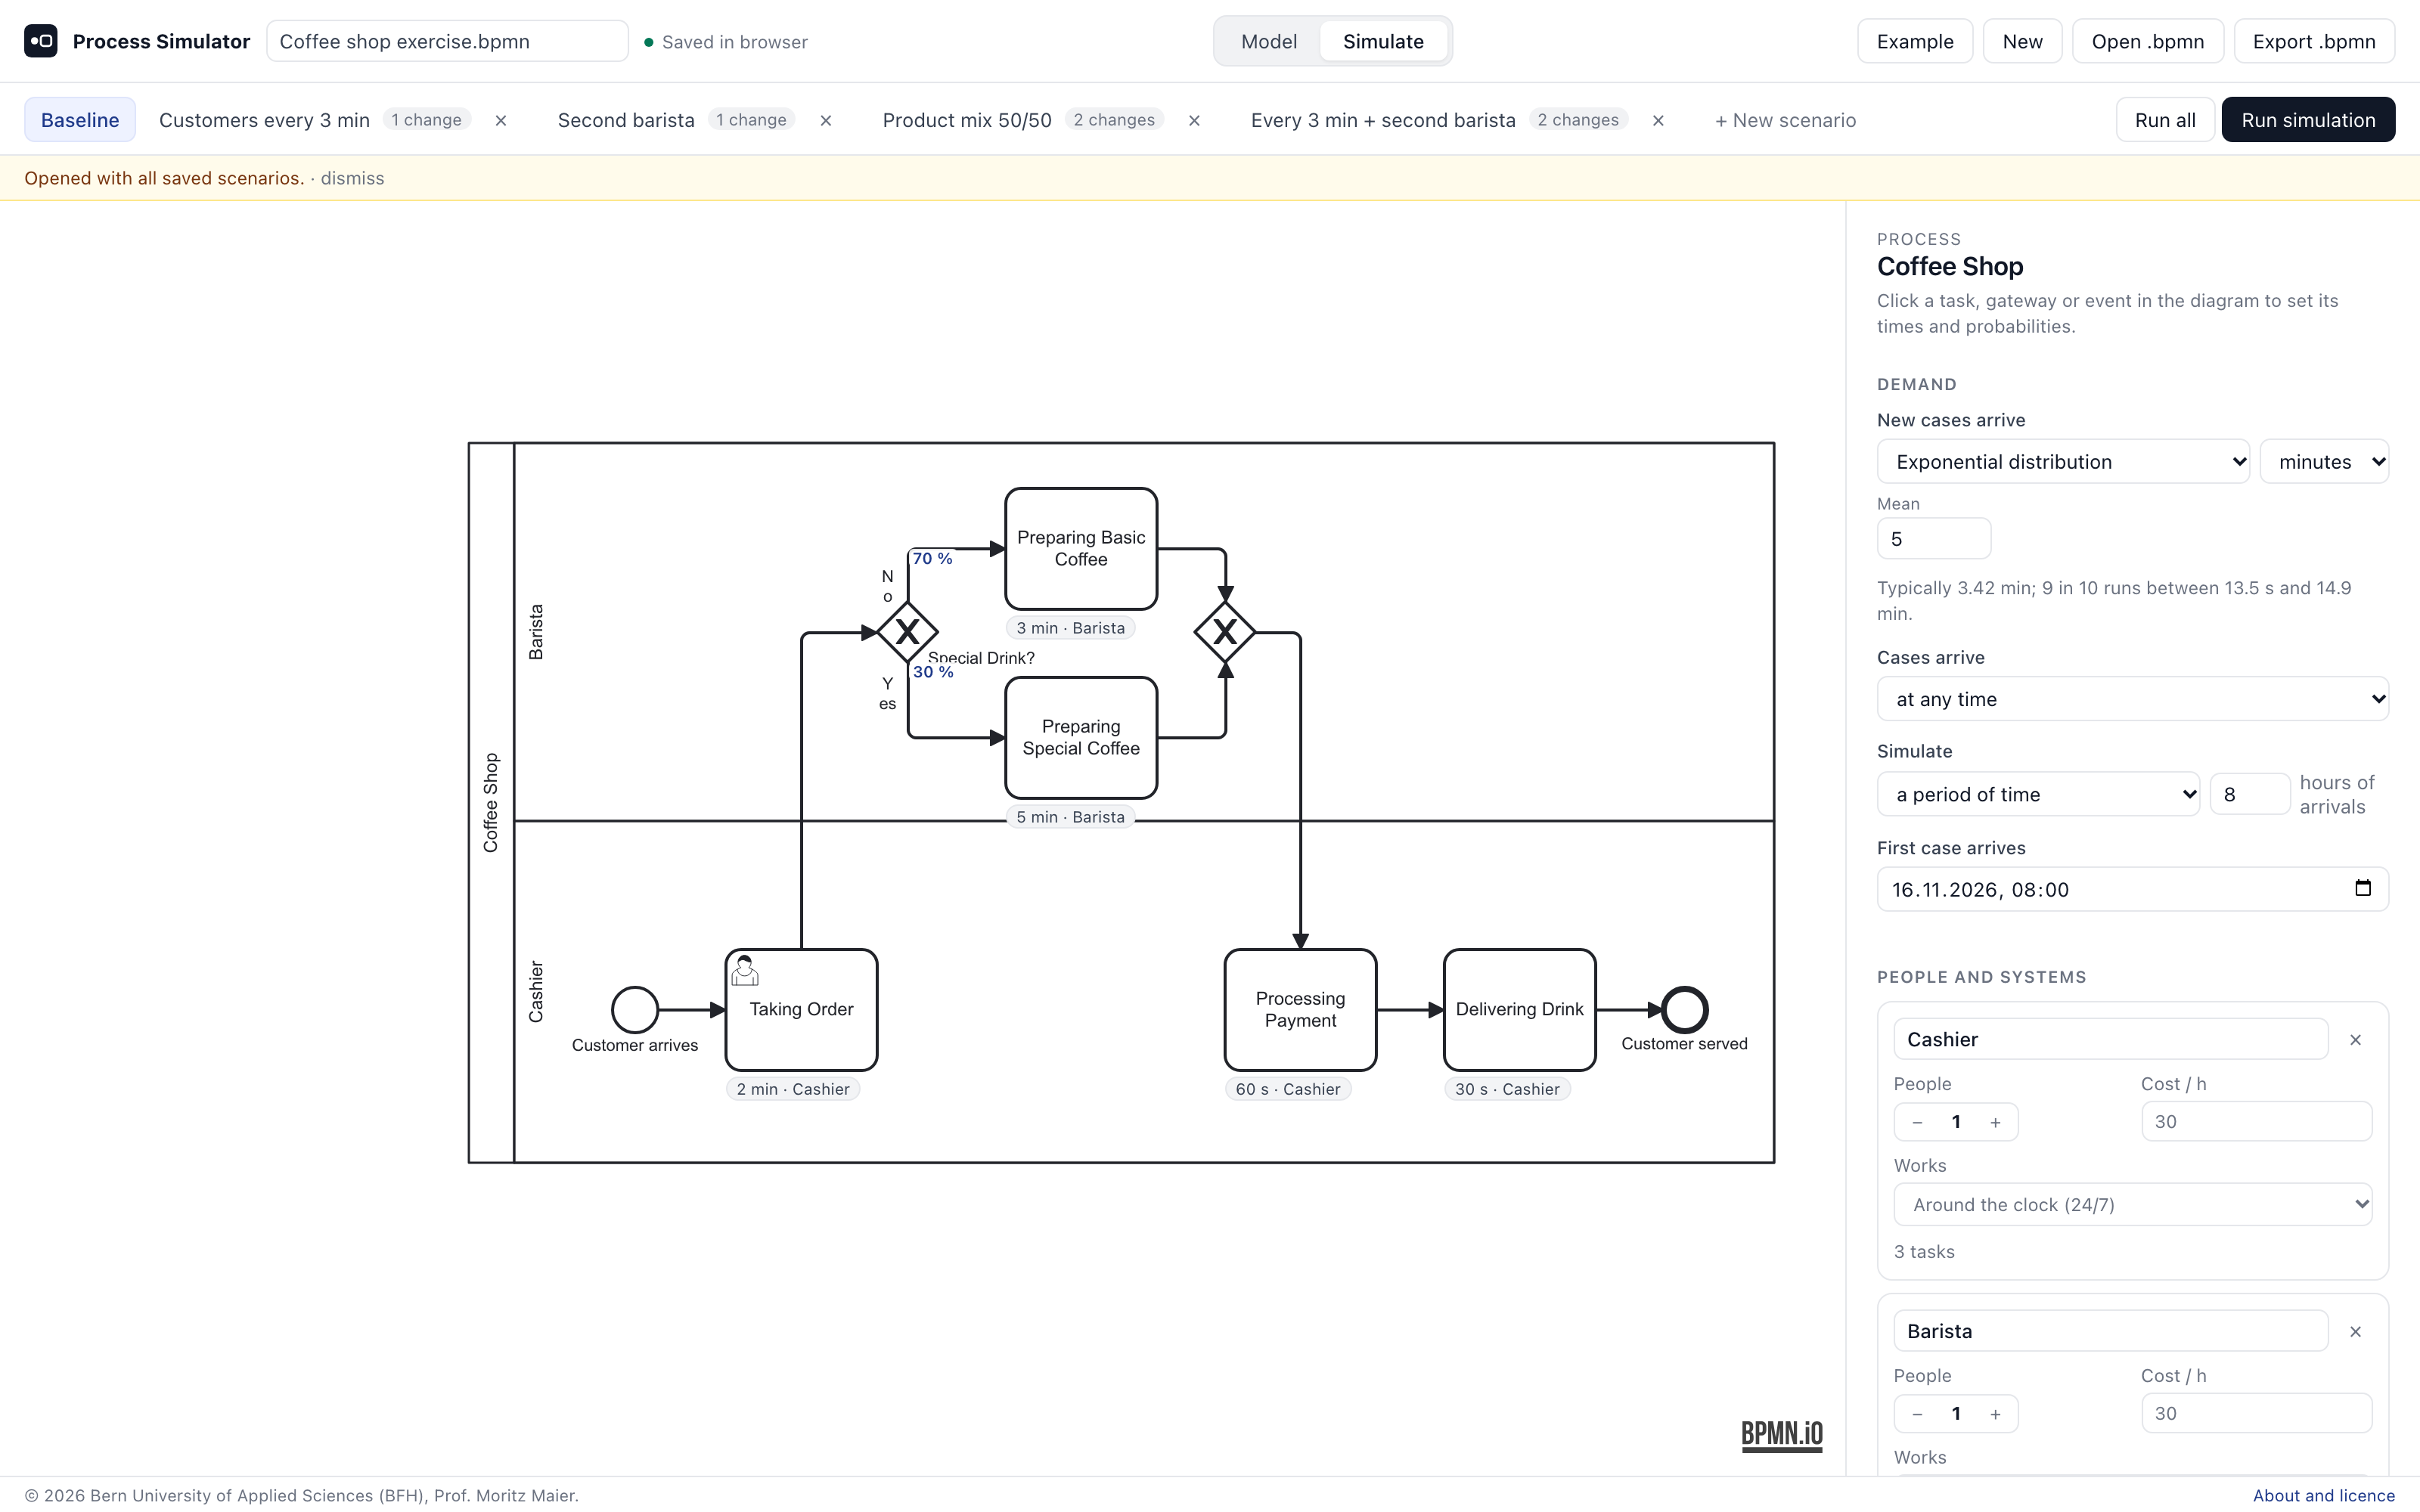
\includegraphics[width=\linewidth]{figures/app-simulate}
\caption{\tool{} in the browser on the shipped coffee-shop example. Above the diagram, tabs switch between the baseline and the stored what-if scenarios; activity annotations show duration and role; the inspector edits the arrival process, resource pools and per-activity parameters of the selected scenario.}
\label{fig:app}
\end{figure}

\tool{} is a TypeScript application. The modeller is bpmn-js; simulation parameters are stored inside the BPMN file as an extension element, so a model and its scenarios travel as one file. The discrete-event engine has no browser dependencies and runs in a Web Worker in the browser, in the Camunda Modeler plugin and in Node.js through the command-line runner \texttt{procsim}. The runner reads a BPMN file, runs one or all stored scenarios, or a scenario given as JSON, for a given number of replications, and writes one JSON line per run with the simulator version, truncated SHA-256 hashes of the model and the scenario, the seed, the replication index and the random-number mode. It also exports scenarios to Prosimos parameters and imports Prosimos parameters, e.g.\ from Simod.

\subsection{Simulation model}
A scenario specifies the arrival process (inter-arrival distribution and optionally a calendar of the hours during which cases arrive), the number of cases or a time horizon, roles with a number of resources, an hourly rate and a weekly working-hours calendar, and for each activity a duration distribution (fixed, exponential, uniform, triangular, normal, lognormal or gamma), a role, an optional cost per run, revenue, queue limit, repetition probability and value class (value-added VA, business-value-added BVA or non-value-added NVA). Branch probabilities are set on the outgoing flows of exclusive and inclusive gateways. The engine executes BPMN token semantics for sequence flows, exclusive, inclusive, parallel, complex and event-based gateways, embedded sub-processes, multi-instance activities, intermediate timer and message events and boundary events. Activities wait in a first-come-first-served queue for a free resource of their role; work outside the calendar is paused and resumed at the next opening. Results include cycle, waiting and processing times (mean and percentiles), throughput, work in progress, utilisation per role, cost and revenue, per-activity statistics and a simulated event log.

\subsection{Statistical scenario comparison}
\label{sec:stats}
Each scenario is simulated in $R$ independent replications (default ten); replication $i$ of every scenario uses the same seed $s_i$. In the default \emph{keyed} mode, every random draw comes from a stream identified by its source (arrival, activity, gateway, boundary event or repetition), the case number and the index of the invocation: the $n$-th time a source is asked for randomness within a case, a small-state generator (sfc32) is seeded with a 32-bit hash of the replication seed, the source key, the case and $n$. A change to one activity therefore leaves the arrival times, branch decisions and durations of all other sources unchanged, and loops keep their draws synchronised per visit. Per-source streams are our implementation choice for CRN, not a requirement of CRN itself \citep{nelson1995}: their purpose is synchronisation of corresponding stochastic events across scenarios. Synchronisation can still degrade when a structural change alters how often a source is visited within a case (for example a new loop), because subsequent invocations of that source shift index; draws of untouched sources remain paired. Also, hash-seeded streams are deterministic by construction; their statistical independence is assumed, not proven. A legacy mode with a single stream for everything is kept for comparison (Section~\ref{sec:v5}).

A run ends when the requested number of cases has arrived (or when a set time horizon is reached); cases still in progress then do not enter the statistics, which restricts them to completed cases. A safety cap on the number of events stops pathological runs and surfaces as a warning in the output. Warm-up is specified as simulated time; cases that arrive before the end of the warm-up are excluded from all statistics.

For each output measure the tool reports the mean over replications with a 95\,\% Student-$t$ confidence interval. Scenarios are compared with the baseline by the paired differences $d_i = Y_i^{\text{scenario}} - Y_i^{\text{baseline}}$; the difference is reported with its confidence interval and marked as not significant when the interval contains zero. These intervals support pairwise estimation; they do not provide simultaneous error control across several alternatives, nor a guaranteed selection of the best one (Section~\ref{sec:v5} quantifies the consequences). The same intervals appear in the app, in the PDF and Excel reports and in the JSON output.

\subsection{Simulation-based value stream mapping}
\label{sec:vsm}
For every completed case the engine records the intervals in which an activity of the case was being processed, together with the value class of the activity and whether the execution was a repetition (rework). The lead time of the case is then partitioned by sweeping its time line. Formally, let $T_c$ be the lead time of case $c$ and $I_{c,k}(t)$ indicate whether at least one activity of category $k$ of case $c$ is in process at time $t$. With the precedence order $\text{VA} \prec \text{BVA} \prec \text{rework} \prec \text{NVA}$, each instant is assigned to
\begin{equation}
g_c(t) = \min_{\prec}\{k : I_{c,k}(t) = 1\},
\end{equation}
and to waiting when no activity is in process. The time attributed to category $k$ is
\begin{equation}
T_{c,k} = \int_0^{T_c} \mathbf{1}[g_c(t) = k]\,dt,
\qquad\text{so that}\qquad
\sum_k T_{c,k} = T_c.
\end{equation}
The partition is unique given the chosen precedence order; the order itself is a modelling decision, not dictated by Lean theory. With parallel branches, an instant in which a VA activity and an NVA activity run simultaneously counts as VA: the NVA work remains visible in the per-activity statistics but does not extend the lead time.

Two consequences deserve emphasis. First, this PCE measures the share of elapsed case time covered by value-adding work, which differs from the work-content share of VA effort: when VA and NVA work overlap, all elapsed time counts as VA while resources also consume NVA effort (Section~\ref{sec:v4} includes a case built to expose this). Second, the precedence rule makes the figures invariant to how work is decomposed into activities along parallel branches, but sensitive to the value classes assigned by the modeller. The value stream view reports the mean of each category, the process cycle efficiency $\text{PCE} = \text{VA}/\text{lead time}$ and the per-activity contributions; it also shows the classical linear figure, the sum of the activity times along the model, to make the difference visible. Figure~\ref{fig:vsm} shows the view on the simulated coffee-shop baseline.

\begin{figure}[t]
\centering
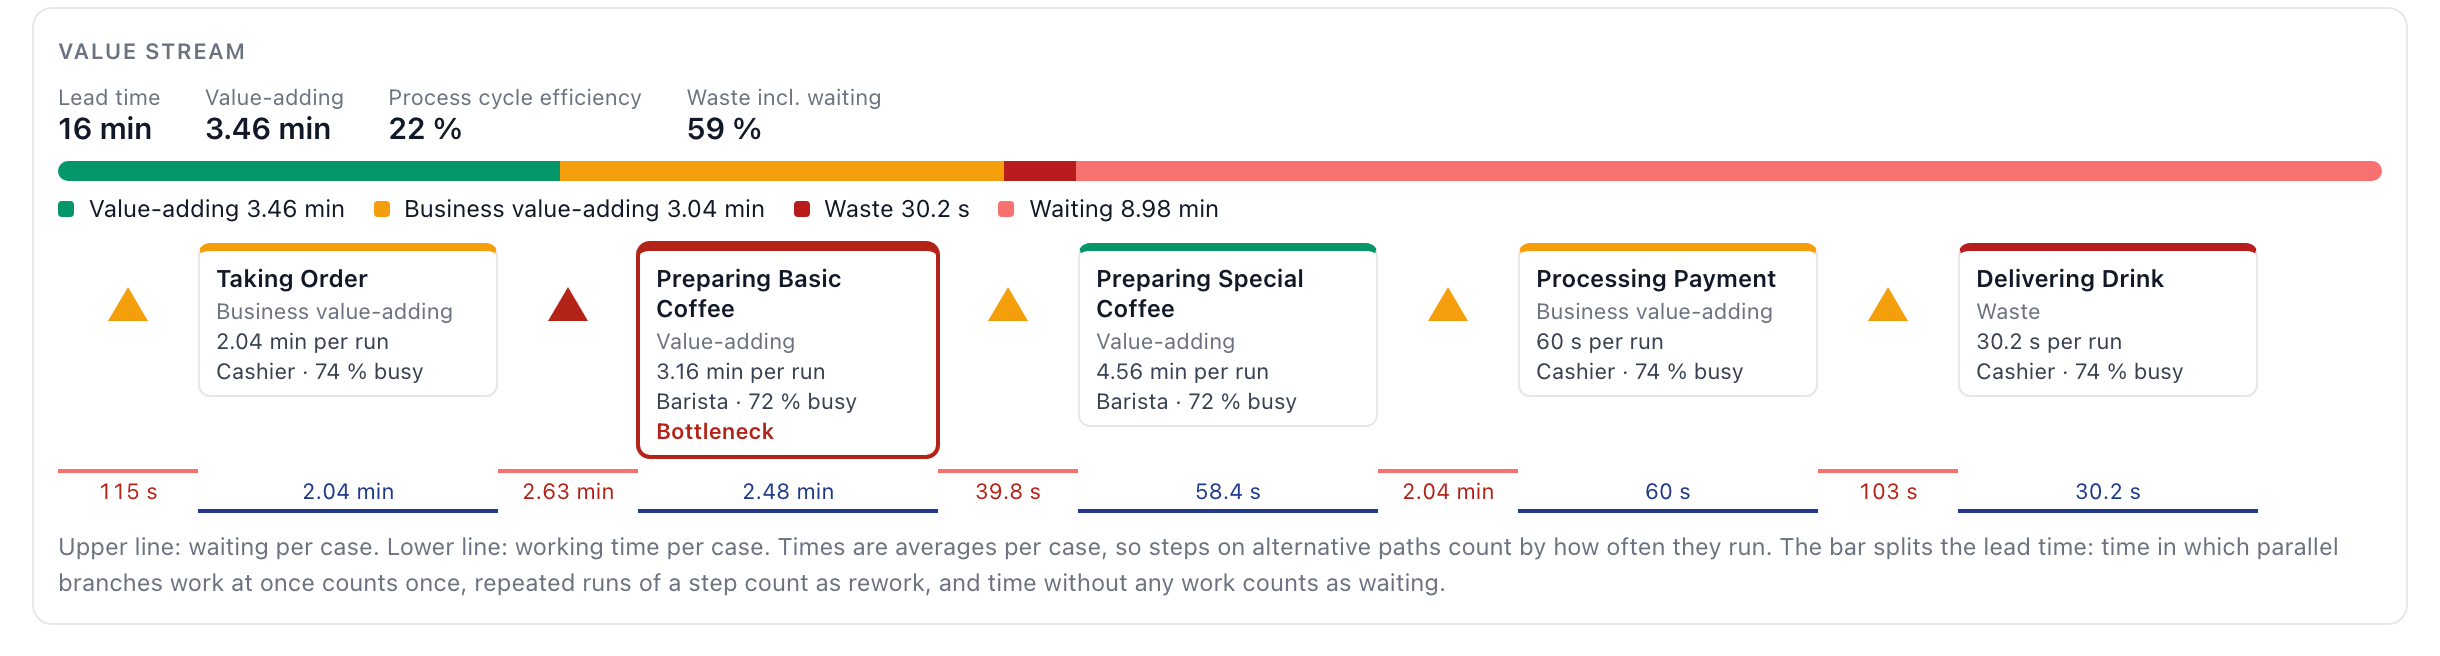
\includegraphics[width=\linewidth]{figures/value-stream}
\caption{Simulation-based value stream map of the coffee-shop example. The bar partitions the mean lead time of 16\,min into value-adding, business-value-adding, waste and waiting; the bottleneck activity is marked. Below, the upper line gives waiting and the lower line working time per activity. A linear map would add the durations of both coffee branches and report a higher PCE than the simulated 22\,\%.}
\label{fig:vsm}
\end{figure}

\section{Evaluation}
\label{sec:eval}
All experiments use the command-line runner of version 1.0.1 and are scripted in the paper repository; \texttt{make} recomputes data, tables and figures. Unless stated otherwise, 95\,\% confidence intervals are Student-$t$ intervals over independent replications. The order of the experiments follows the question that opened this paper: Sections~\ref{sec:v1}--\ref{sec:v4} establish that the engine and its value stream figures can be trusted, Section~\ref{sec:v5} measures how often the single-run shortcut fails, and Sections~\ref{sec:v6}--\ref{sec:v7} place run time and feature coverage in context. We distinguish \emph{verification} (does the engine implement the intended model correctly?), \emph{cross-engine consistency} (does it agree with an independent implementation?) and \emph{model fidelity} (does the simulated model reproduce a real process?); the experiments address the first two, not the third. \ref{app:models} shows the test models.

\subsection{V1: does the engine reproduce exact queueing results?}
\label{sec:v1}
We built BPMN models whose steady-state behaviour is known analytically: M/M/1 at utilisation $\rho\in\{0.5,0.8,0.9\}$, M/M/3 and M/M/10, M/D/1, M/U/1 and M/G/1 with lognormal and gamma service (Pollaczek--Khinchine), a tandem of two M/M/1 stations and a Jackson network with feedback \citep{jackson1957}. Each case ran \VoneReps{} replications of \VoneCases{} cases with a warm-up of 2000 mean inter-arrival times. Table~\ref{tab:v1} compares the simulated mean waiting time (or cycle time) with the exact value. All \VoneCovered{} intervals contain the exact value, and the largest relative error is \VoneWorst. With correct marginal coverage about 12.4 of 13 intervals would be expected to cover the truth, so the observed result is consistent with nominal coverage without proving it. Little's law $L=\lambda W$ \citep{little1961}, computed from the reported work in progress, throughput and cycle time, holds within \VoneLittle.

\begin{table}[t]
\centering\small
\caption{V1: simulated versus exact mean times in seconds; 13 verification quantities across the tested models.}
\label{tab:v1}
\resizebox{\linewidth}{!}{\begin{tabular}{llrrrc}
\toprule
Model & Quantity & Exact & Simulated (95\,\% CI) & Error & In CI \\
\midrule
M/M/1, $\rho$=0.5 & mean wait & 30.0 & 30.0 $\pm$ 0.2 & -0.14\,\% & yes \\
M/M/1, $\rho$=0.8 & mean wait & 192.0 & 191.4 $\pm$ 2.5 & -0.33\,\% & yes \\
M/M/1, $\rho$=0.9 & mean wait & 486.0 & 483.8 $\pm$ 13.0 & -0.46\,\% & yes \\
M/M/3, $\rho$=0.8 & mean wait & 155.3 & 154.9 $\pm$ 2.5 & -0.24\,\% & yes \\
M/M/10, $\rho$=0.9 & mean wait & 361.1 & 360.7 $\pm$ 13.1 & -0.11\,\% & yes \\
M/D/1, $\rho$=0.8 & mean wait & 96.0 & 95.9 $\pm$ 0.9 & -0.10\,\% & yes \\
M/U/1, $\rho$=0.8 & mean wait & 104.0 & 104.1 $\pm$ 0.9 & +0.09\,\% & yes \\
M/G/1 lognormal cv=1.5, $\rho$=0.8 & mean wait & 312.0 & 311.4 $\pm$ 7.6 & -0.19\,\% & yes \\
M/G/1 gamma cv=0.5, $\rho$=0.8 & mean wait & 120.0 & 119.8 $\pm$ 1.1 & -0.15\,\% & yes \\
Tandem M/M/1 to M/M/1 & mean wait station 1 & 80.0 & 79.8 $\pm$ 0.6 & -0.25\,\% & yes \\
Tandem M/M/1 to M/M/1 & mean wait station 2 & 192.0 & 190.4 $\pm$ 2.7 & -0.86\,\% & yes \\
Jackson feedback, p=0.25 & mean wait per visit & 144.0 & 143.9 $\pm$ 1.7 & -0.06\,\% & yes \\
Jackson feedback, p=0.25 & mean time in system & 240.0 & 239.8 $\pm$ 2.3 & -0.07\,\% & yes \\
\bottomrule
\end{tabular}
}
\end{table}

\subsection{V2: do the engines agree on shared semantics?}
\label{sec:v2}
Five models (tandem, M/M/3, exclusive choice, parallel split and rework loop) were exported with the built-in converter and simulated by Prosimos 2.1.0 and by \tool{}, \VtwoReps{} replications of \VtwoCases{} cases each. The two engines use different random-number generators, so we compare means. Table~\ref{tab:v2} lists the relative difference with a Welch confidence interval. The intervals contain zero for \VtwoZero{} quantities, but a confidence interval covering zero does not establish equivalence. We therefore apply an equivalence margin of $\pm5$\,\%, chosen as a difference that would be operationally negligible next to typical model-specification error: \VtwoEquiv{} intervals lie fully inside the margin, and the widest admits differences up to \VtwoBound{} (the waiting time of the three-server model). Eleven of the thirteen point estimates of \tool{} are slightly higher (by 0.7--2.5\,\%), so a small systematic difference cannot be excluded at this sample size; it is of the order of the interval half-widths. The data bound the difference between the engines to a few percent on the shared semantics; they do not show that either engine is correct. Features without a Prosimos counterpart, such as queue limits, revenue or boundary events, are listed by the exporter and were not used. One larger example model, the coffee shop shipped with the tool, could not be run by Prosimos (an internal error in its control-flow handling), which we report as a limitation of the cross-check.

\begin{table}[t]
\centering\small
\caption{V2: \tool{} versus Prosimos, mean times in seconds and relative difference with 95\,\% confidence interval.}
\label{tab:v2}
\resizebox{\linewidth}{!}{\begin{tabular}{llrrr}
\toprule
Model & Quantity & This tool & Prosimos & Difference (95\,\% CI) \\
\midrule
Sequence, two M/M/1 stations & mean cycle time & 360.6 & 357.7 & +0.8\,\% [-1.2, +2.8] \\
Sequence, two M/M/1 stations & mean wait t1 & 80.1 & 79.6 & +0.7\,\% [-1.4, +2.7] \\
Sequence, two M/M/1 stations & mean wait t2 & 192.5 & 190.1 & +1.3\,\% [-2.0, +4.5] \\
One activity, three servers & mean cycle time & 301.3 & 298.7 & +0.9\,\% [-1.3, +3.1] \\
One activity, three servers & mean wait t1 & 157.3 & 154.5 & +1.8\,\% [-2.2, +5.9] \\
Exclusive choice 30/70, shared role & mean cycle time & 289.2 & 292.1 & -1.0\,\% [-3.7, +1.8] \\
Exclusive choice 30/70, shared role & mean wait a & 236.5 & 239.7 & -1.3\,\% [-4.7, +2.1] \\
Exclusive choice 30/70, shared role & mean wait b & 237.4 & 240.2 & -1.2\,\% [-4.5, +2.1] \\
Parallel split, two roles & mean cycle time & 246.6 & 242.8 & +1.6\,\% [-0.4, +3.5] \\
Parallel split, two roles & mean wait a & 136.0 & 133.4 & +1.9\,\% [-0.9, +4.7] \\
Parallel split, two roles & mean wait b & 141.8 & 138.3 & +2.5\,\% [-0.3, +5.3] \\
Rework loop p = 0.25 & mean cycle time & 243.8 & 239.8 & +1.7\,\% [-0.6, +4.0] \\
Rework loop p = 0.25 & mean wait work & 146.8 & 143.8 & +2.1\,\% [-0.7, +5.0] \\
\bottomrule
\end{tabular}
}
\end{table}

\subsection{V3: does the engine stay consistent on a discovered model?}
\label{sec:v3}
To exercise the engine on realistic input we used the BPI Challenge 2012 log \citep{bpic2012}, restricted to the work items (activities starting with \texttt{W\_}) with start and completion events, i.e.\ \VthreeCases{} cases. Simod 5.2.1 \citep{camargo2020} discovered a BPMN model with branching probabilities, resource profiles, calendars and duration distributions. Prosimos simulated this model directly; \tool{} imported the Prosimos parameters. Because \tool{} has one role and one duration per activity, the importer pools roles that share activities and merges the resource-specific durations of an activity into a gamma distribution with the same mean and variance; it reports \VthreeApprox{} such approximations. Table~\ref{tab:v3} compares both engines with the log. The mean cycle times of the two engines differ by \VthreeDiff; since Prosimos simulated the original model and \tool{} its imported approximation, this figure bounds the combined effect of the import approximations and any remaining semantic difference. Both engines also produce about 17.9 work items per case against 7.4 in the log, so the discovered control flow repeats activities far more often than the real process; the two engines agree with each other on this as well. The cycle times of both engines are far below the cycle time in the log, because the discovered model does not represent the time cases spend waiting outside the recorded work items; this is a property of the discovered model, not of either engine, and illustrates the threats discussed by \citet{bluemel2026}. This experiment is therefore a consistency test between two implementations on realistic input, not a validation of predictive fidelity against the log.

\begin{table}[t]
\centering\small
\caption{V3: BPI Challenge 2012 work items, log versus simulation of the discovered model, ten replications each (mean $\pm$ half-width of the 95\,\% confidence interval).}
\label{tab:v3}
\IfFileExists{generated/v3_table.tex}{\begin{tabular}{lrrr}
\toprule
Measure & Log & Prosimos & This tool \\
\midrule
mean cycle time (h) & 252.02 & 3.42 $\pm$ 0.05 & 3.40 $\pm$ 0.03 \\
work items per case & 7.39 & 17.86 $\pm$ 0.07 & 17.80 $\pm$ 0.06 \\
\bottomrule
\end{tabular}
}{}
\end{table}

\subsection{V4: are the value stream figures correct for non-linear processes?}
\label{sec:v4}
Seven models with closed-form lead time and partition were simulated with \VfourReps{} replications: a sequence of three activities, an exclusive choice (30/70), a parallel split, a parallel split with value-adding and non-value-adding work of equal duration, a composite of a choice, a parallel pair and a rework loop, a rework loop with repetition probability 0.5 and a tandem with queues. Table~\ref{tab:v4} compares lead time and PCE with the exact values and with the PCE of a linear value stream map that adds the activity times along the model. The simulated figures agree with the exact ones within sampling error, and in every case the categories add up to the lead time (largest deviation $\VfourPartition$\,s). The linear map overstates PCE for the choice (because it adds both branches), understates it for the parallel split (because it adds parallel work) and ignores rework. The equal-duration case makes the semantics of the partition explicit: the simulated PCE is 1.0 although half of the work content is non-value-adding, because every instant of elapsed time carries VA work; the NVA effort is reported in the activity statistics but does not extend the lead time.

\begin{table}[t]
\centering\small
\caption{V4: lead time (s), PCE and rework time (s): exact, simulated and from a linear value stream map.}
\label{tab:v4}
\resizebox{\linewidth}{!}{\begin{tabular}{lrrrrrr}
\toprule
Case & \multicolumn{2}{c}{Lead time} & \multicolumn{3}{c}{PCE} & Rework \\
 & exact & tool & exact & tool & linear map & tool \\
\midrule
Sequence & 60.0 & 60.0 & 0.167 & 0.167 & 0.167 & 0.0 \\
Exclusive choice (30/70) & 58.0 & 57.9 & 0.517 & 0.515 & 0.714 & 0.0 \\
Parallel split & 50.0 & 50.0 & 1.000 & 1.000 & 0.625 & 0.0 \\
Rework loop (p = 0.5) & 40.0 & 39.9 & 0.500 & 0.502 & 1.000 & 19.9 \\
Sequence with queues (M/M/1 tandem) & 360.0 & 358.1 & 0.111 & 0.112 & -- & 0.0 \\
\bottomrule
\end{tabular}
}
\end{table}

\subsection{V5: single runs versus replications}
\label{sec:v5}
We return to the question that opened this paper: which option is best, and how often does one run per option answer it wrongly? We took two decision problems: the coffee-shop example (four alternatives to the baseline) and an office process with a baseline and four staffing and duration options. The reference ranking comes from an independent high-precision run: \VfiveRef{} replications per option in a seed block disjoint from the trials, so no replication contributes to both the reference and the evaluated decisions. In both problems the best option leads the runner-up by a clearly resolved margin (21.8\,\% and 9.8\,\% of mean cycle time). We then repeated, \VfiveN{} times, the decision ``pick the option with the lowest mean cycle time'', sweeping the budget from one run per option to groups of up to 50 paired replications; Table~\ref{tab:v5} reports the share of correct selections with Wilson intervals. With one run per option the answer is wrong in \VfiveCoffeeIndep{} of trials on the coffee shop and \VfiveOfficeIndep{} on the harder office problem when seeds are independent; per-source streams (keyed mode) reduce this to \VfiveOfficeKeyed, and a shared single stream to \VfiveOfficeSingle. Five paired replications already decide correctly in 99.5\,\% of office trials; ten or more are correct in every observed trial. The paired confidence intervals of the tool never declared a wrong direction and returned ``not significant'' in at most \VfiveNs{} of the comparisons with the baseline. Table~\ref{tab:v5var} shows why: per-source streams reduce the variance of differences by up to a factor of \VfiveRatio{} compared with a single stream. For the coffee-shop owner of the introduction this is the difference between acting on a coin flip and acting on evidence: two paired runs already answer correctly in every observed trial, and the intervals say when evidence is missing rather than inventing it.

\begin{table}[t]
\centering\small
\caption{V5: share of \VfiveN{} independent decision trials in which the truly best option was chosen, by random-number mode and replication budget per option; brackets give the 95\,\% Wilson interval. The reference ranking uses a disjoint set of \VfiveRef{} replications per option.}
\label{tab:v5}
\resizebox{\linewidth}{!}{\begin{tabular}{lrrrr}
\toprule
Problem & \multicolumn{3}{c}{One run per scenario} & 10 paired runs \\
 & one stream, same seed & per-source streams & independent seeds & mean \\
\midrule
Coffee shop & 99.7\,\% & 100.0\,\% & 80.7\,\% & 100.0\,\% \\
Office process & 73.7\,\% & 80.2\,\% & 54.9\,\% & 99.5\,\% \\
\bottomrule
\end{tabular}
}
\end{table}

\begin{table}[t]
\centering\small
\caption{V5: variance of the difference to the baseline in mean cycle time (s$^2$) for one run per option.}
\label{tab:v5var}
\resizebox{\linewidth}{!}{\begin{tabular}{llrrrr}
\toprule
Problem & Option & True difference (s) & \multicolumn{3}{c}{Variance of the difference} \\
 & & & independent & one stream & per source \\
\midrule
Coffee shop & Customers every 3 min & +951.5 & 327173 & 279529 & 254513 \\
Coffee shop & Second barista & -157.2 & 28334 & 11993 & 10595 \\
Coffee shop & Product mix 50/50 & +183.1 & 102702 & 41657 & 30029 \\
Coffee shop & Every 3 min + second barista & +157.8 & 28119 & 20395 & 18007 \\
Office process & Second person at step 1 & -179.2 & 17446 & 6128 & 3190 \\
Office process & Step 2 10 \% faster & -116.4 & 16098 & 4298 & 1822 \\
Office process & Step 3 11 \% faster & -58.2 & 19834 & 4660 & 231 \\
Office process & Second person at step 3 & -124.6 & 18939 & 5545 & 649 \\
\bottomrule
\end{tabular}
}
\end{table}

\subsection{V6: how does run time scale?}
\label{sec:v6}
Run time measures the implementation on a given machine, not the tool as such: it depends on the processor, the JavaScript engine and the load on the machine, whereas the simulated results do not. We therefore ran the same workloads on one machine (\VsixCpu, 8 threads) with the command-line runner (Node.js \VsixNode) and with the engine in a Web Worker, as in the web application, in headless Chromium and Firefox. Each point is the median of \VsixReps{} replications and times the simulation only, not loading the model; Firefox reports these times in whole milliseconds. The engine's safety cap on the number of events was raised via the runner's \texttt{--max-events} option so that every requested case ran to completion. For the same seeds all three runtimes produced identical results (\VsixMismatches{} differences in \VsixCompared{} comparisons). Figure~\ref{fig:v6} shows that run time grows approximately linearly with the number of cases; one million cases of a one-activity process take \VsixMillion\,s in Node.js (about \VsixRate{} cases per second), \VsixMillionChromium\,s in Chromium and \VsixMillionFirefox\,s in Firefox. Run time grows slightly faster than linearly with the number of activities or parallel branches per case, since every token event is a heap operation on a larger event list and more per-activity statistics are kept. Across all workloads the browsers took between \VsixRatioMin{} and \VsixRatioMax{} times as long as Node.js. On other hardware the absolute times will differ, but the scaling is a property of the engine.

\begin{figure}[t]
\centering
\IfFileExists{generated/v6_performance.pdf}{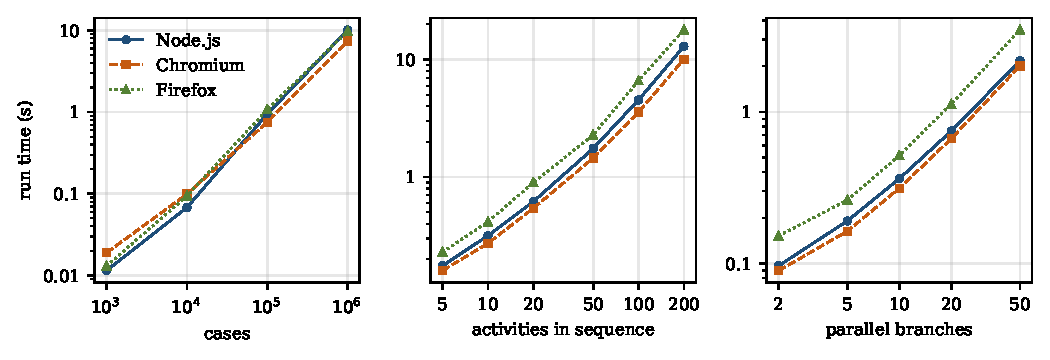
\includegraphics[width=\linewidth]{generated/v6_performance}}{}
\caption{V6: run time by number of cases, sequence length and number of parallel branches, in Node.js and in a Web Worker in Chromium and Firefox on the same machine (logarithmic axes; median of \VsixReps{} replications).}
\label{fig:v6}
\end{figure}

\subsection{V7: how does the tool compare with existing ones?}
\label{sec:v7}
Table~\ref{tab:v7} positions \tool{} against two openly documented research tools that serve the same purpose, BIMP (the online front end of the QBP simulator) and Prosimos with Simod. Browser access alone is not the differentiator: both other tools can be reached through a web interface. What distinguishes \tool{} is the integration of modelling, simulation, replicated comparison and the value stream view in one browser application, and its particular statistical and VSM features. The entries for Prosimos were checked against the source code of release 2.1.0, the latest at the time of writing (command-line options, simulation API and random-number generation), and against its web service; the entries for BIMP come from its public documentation and its open-source user interface, as the QBP engine itself is not published. All sources were consulted in November 2026. ``Not documented'' means that the feature appears neither in the documentation nor in the inspected code, not that it is absent. Commercial suites with simulation modules were not included because their feature sets could not be checked from public sources in a comparable way; surveys of such tools are available \citep{pereira2016,rosenthal2021}.

\begin{table}[!htbp]
\centering\small
\caption{V7: feature comparison based on public documentation and, for Prosimos, the source code of release 2.1.0.}
\label{tab:v7}
\scriptsize
\begin{tabularx}{\linewidth}{@{}>{\raggedright\arraybackslash}p{3.3cm}*{3}{>{\raggedright\arraybackslash}X}@{}}
\toprule
Feature & \tool{} & BIMP (QBP) & Prosimos / Simod \\
\midrule
Runs in the browser, no installation & yes & yes (upload of a BPMN file) & engine in Python; open-source web application available \\
Integrated BPMN editor & yes (bpmn-js, Camunda Modeler plugin) & no, external modeller & no, external modeller \\
Command-line / batch use & yes & not documented & yes \\
Discovery from event logs & no (imports Simod output) & no & yes (Simod) \citep{camargo2020} \\
Differentiated resources (individual calendars and durations) & no, roles & no & yes \citep{lopezpintado2022} \\
Replications with confidence intervals & yes & no; one run per simulation, no replication setting documented & no; one run per call, repeatable only by an external script \\
Common random numbers across scenarios & yes, per-source streams & not documented; engine not published & no per-source streams; one global generator, seedable only from outside \\
Paired scenario comparison & yes & no & no \\
Value stream figures (VA/BVA/NVA, PCE) & yes, simulation-based & no & no \\
Licence & Apache-2.0 & user interface MIT; engine not published & engine: no licence file; web services Apache-2.0 \\
\bottomrule
\end{tabularx}
\end{table}


\section{Discussion and limitations}
\label{sec:discussion}
The verification covers steady-state queueing behaviour, the semantics shared with Prosimos and the VSM partition; it does not cover every BPMN construct the engine executes. Event-based gateways, inclusive gateways, multi-instance activities and boundary events are covered by unit tests but not by an external reference; conformance tests against externally defined traces are future work. The resource model is coarser than that of Prosimos: there are no individual resource calendars, no resource-specific durations, no batching and no prioritisation, so models discovered by Simod have to be approximated (Section~\ref{sec:v3}); the V3 result bounds but does not isolate the effect of these approximations. The tool reports confidence intervals and paired differences but leaves the choice among several significant options to the user; ranking-and-selection procedures \citep{kim2001} would be a natural extension. The decision experiment (V5) uses two decision problems; it demonstrates the effect of single runs under controlled conditions and is not a general estimate of error rates. The VSM categories depend on the value classes assigned by the modeller, the precedence rule for overlapping work is a design choice, and the reported PCE measures elapsed-time coverage rather than work-content share (Sections~\ref{sec:vsm}, \ref{sec:v4}). The hash-seeded random streams are deterministic; their independence is assumed, and structural scenario changes can desynchronise paired draws (Section~\ref{sec:stats}). No user study was conducted, so claims about usability are limited to the tool's availability in the browser and the modeller plugin.

\section{Conclusion}
\label{sec:conclusion}
The question that opened this paper now has a defensible answer: a single run per scenario decides by chance, whereas replicated and paired comparisons decide by evidence. \tool{} brings replicated, CRN-based scenario comparison and value stream figures for non-linear processes into a BPMN editor that runs in the browser and in the Camunda Modeler. The evaluation shows agreement with exact queueing results and with an independent engine, correct VSM figures for choices, parallel branches and loops, and a clear reduction of wrong decisions compared with single runs. The software, the experiments and the data are available under Apache-2.0.

\section*{Software and data availability}
\begin{itemize}\sloppy
\item Software: \url{https://github.com/BFH-Process-Digitalization/process-simulator} (Apache-2.0); web application: \url{https://bfh-process-digitalization.github.io/process-simulator/}. The results reported here were produced with simulator release 1.0.1 (tag \texttt{v1.0.1}).
\item Experiments, generated models, raw runs and this manuscript: \url{https://github.com/BFH-Process-Digitalization/process-simulator-paper}.
\item The BPI Challenge 2012 log is not redistributed; the scripts download it from 4TU.ResearchData \citep{bpic2012}.
\end{itemize}

\section*{CRediT authorship contribution statement}
\textbf{Moritz Maier:} Conceptualization, Software, Validation, Writing -- original draft, Writing -- review \& editing.

\section*{Declaration of competing interest}
The author declares no competing interests.

\section*{Declaration of generative AI and AI-assisted technologies in the writing process}
During the preparation of this work the author used generative AI tools in order to draft and revise parts of the manuscript. After using these tools, the author reviewed and edited the content as needed and takes full responsibility for the content of the publication.

\bibliographystyle{apacite}
\bibliography{references}

\appendix
\setcounter{figure}{0}
\section{Test models}
\label{app:models}
The BPMN models used in V1, V2, V4 and V5 are generated by the model builder in \url{experiments/lib/bpmn.mjs} and stored in the \texttt{models/} directory of the paper repository; Figure~\ref{fig:models} shows them as rendered by bpmn-js. The BPI Challenge 2012 model of Section~\ref{sec:v3} is discovered by Simod 5.2.1 from the event log and regenerated by \texttt{make v3}; it is too large to reproduce legibly here.

\begin{figure}[H]
\centering
\begin{minipage}{.48\linewidth}\centering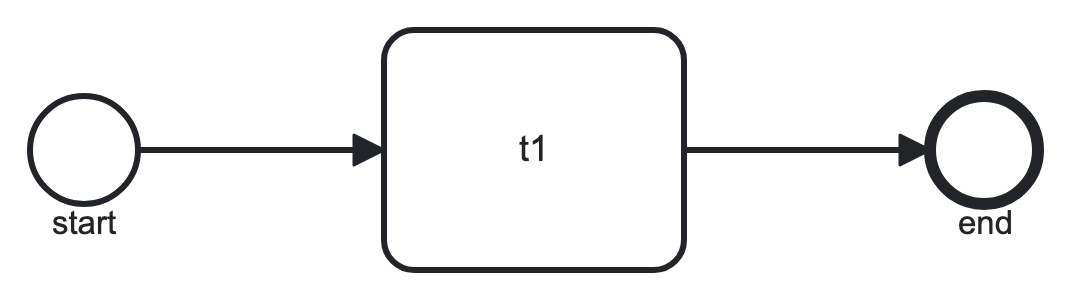
\includegraphics[width=\linewidth]{figures/models/single-station}\\(a) single station (V1)\end{minipage}\hfill
\begin{minipage}{.48\linewidth}\centering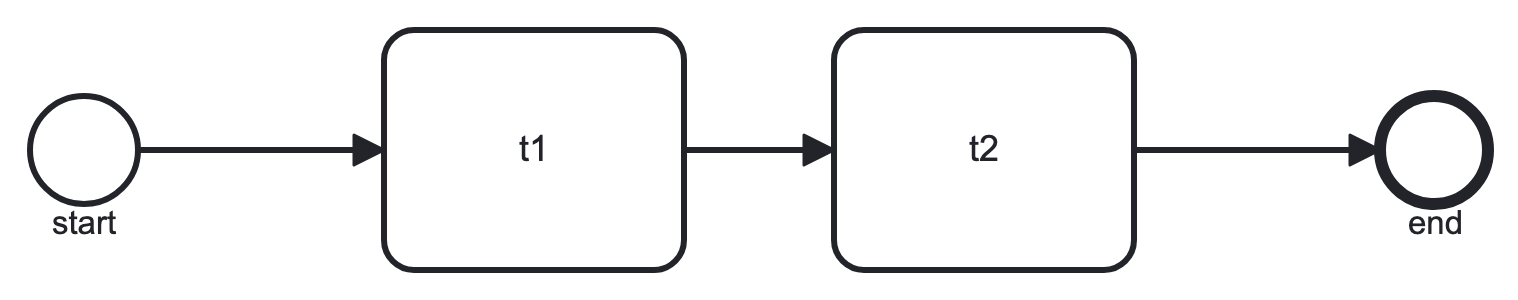
\includegraphics[width=\linewidth]{figures/models/tandem}\\(b) tandem of two stations (V1, V2, V4)\end{minipage}\\[1em]
\begin{minipage}{.48\linewidth}\centering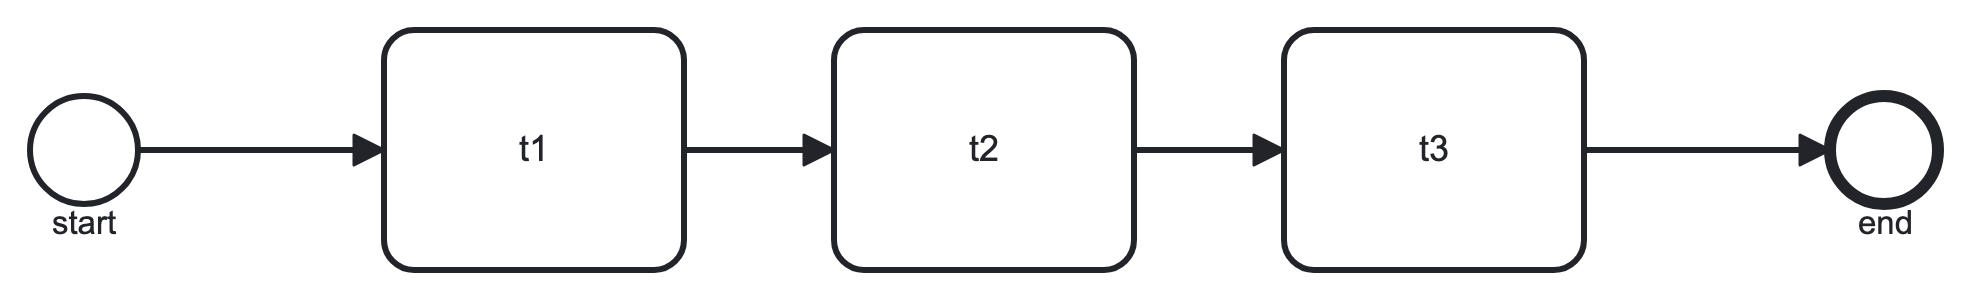
\includegraphics[width=\linewidth]{figures/models/three-step}\\(c) three-step sequence (V4, V5 office process)\end{minipage}\hfill
\begin{minipage}{.48\linewidth}\centering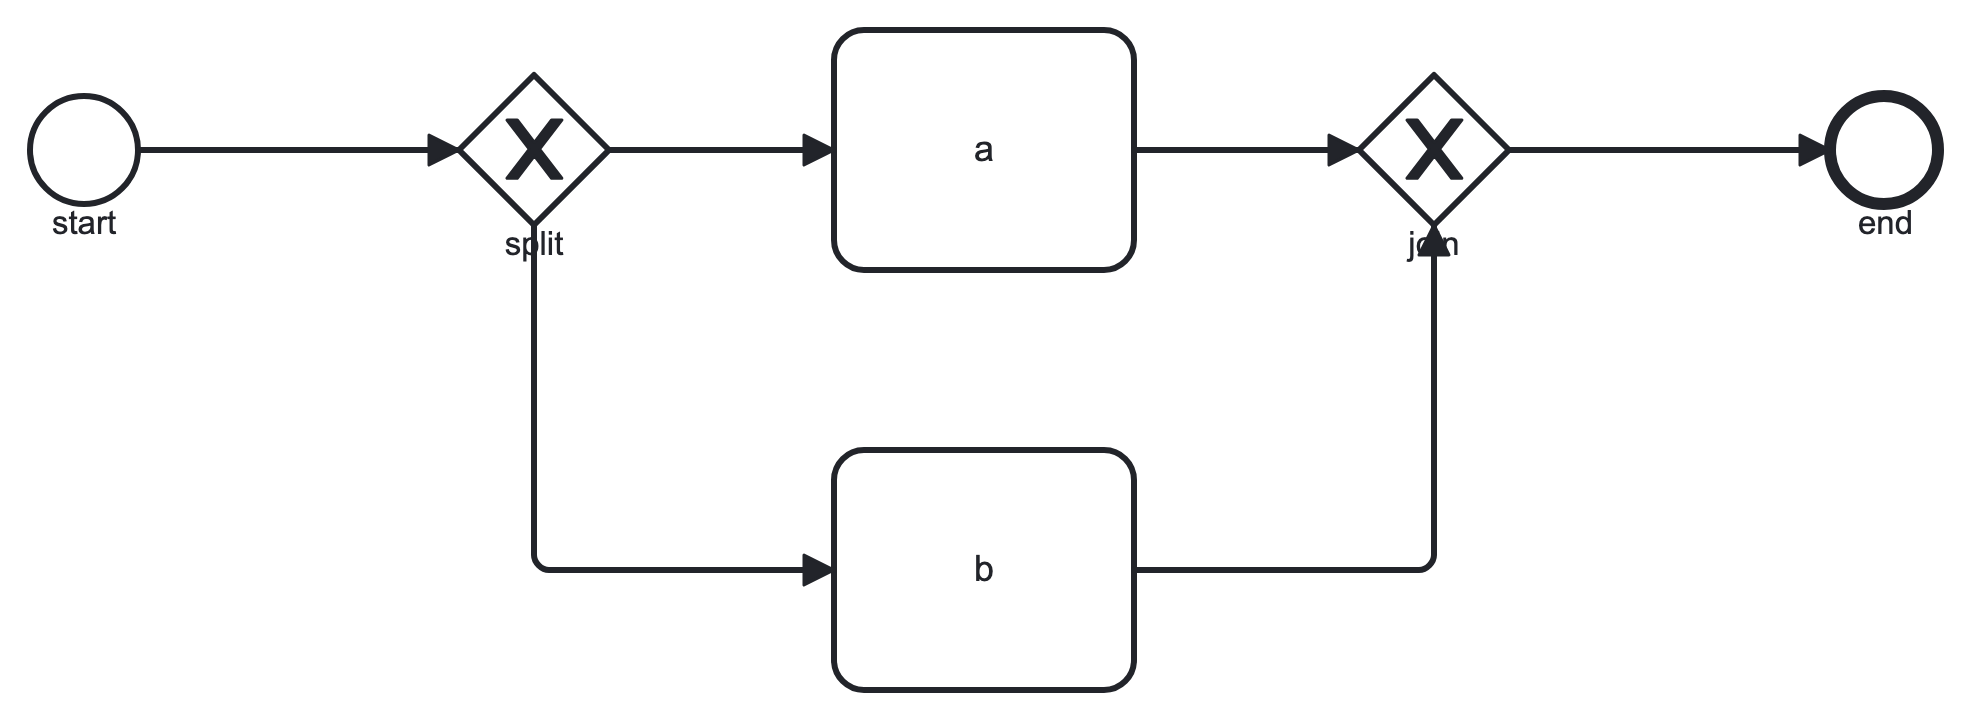
\includegraphics[width=\linewidth]{figures/models/exclusive-choice}\\(d) exclusive choice (V2, V4)\end{minipage}\\[1em]
\begin{minipage}{.48\linewidth}\centering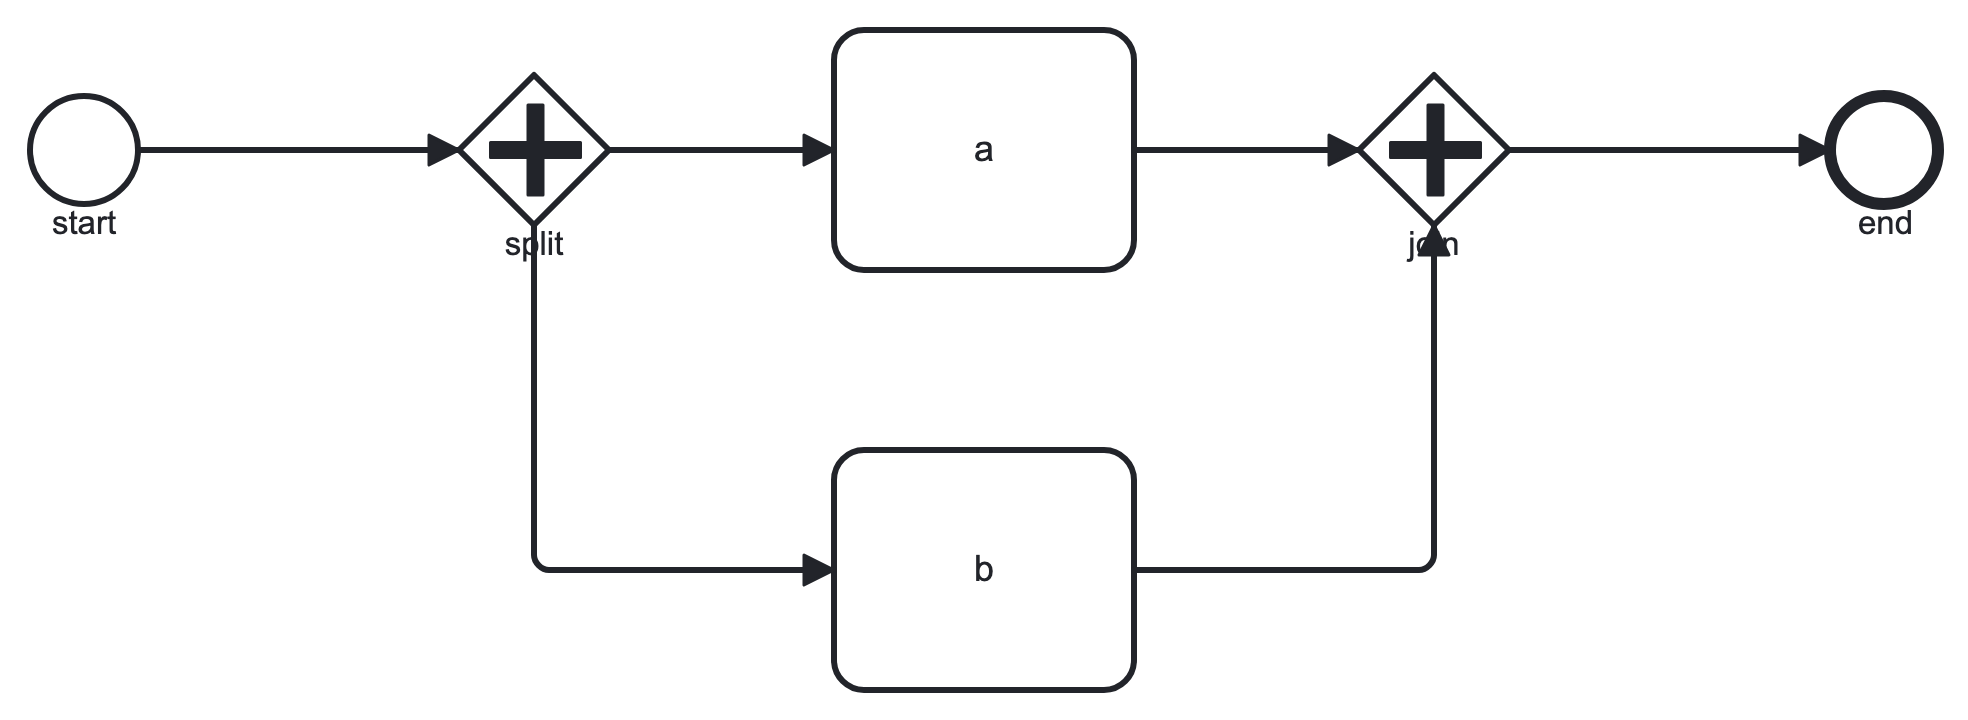
\includegraphics[width=\linewidth]{figures/models/parallel-split}\\(e) parallel split (V2, V4)\end{minipage}\hfill
\begin{minipage}{.48\linewidth}\centering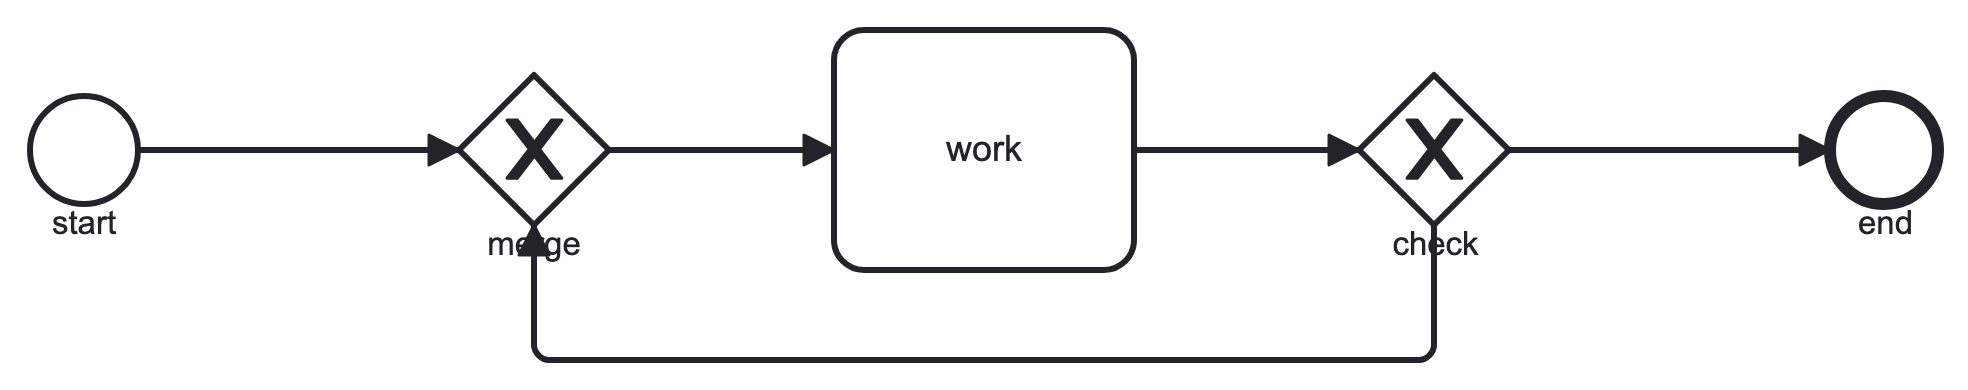
\includegraphics[width=\linewidth]{figures/models/rework-loop}\\(f) rework loop, also the Jackson feedback network (V1, V2, V4)\end{minipage}\\[1em]
\begin{minipage}{.48\linewidth}\centering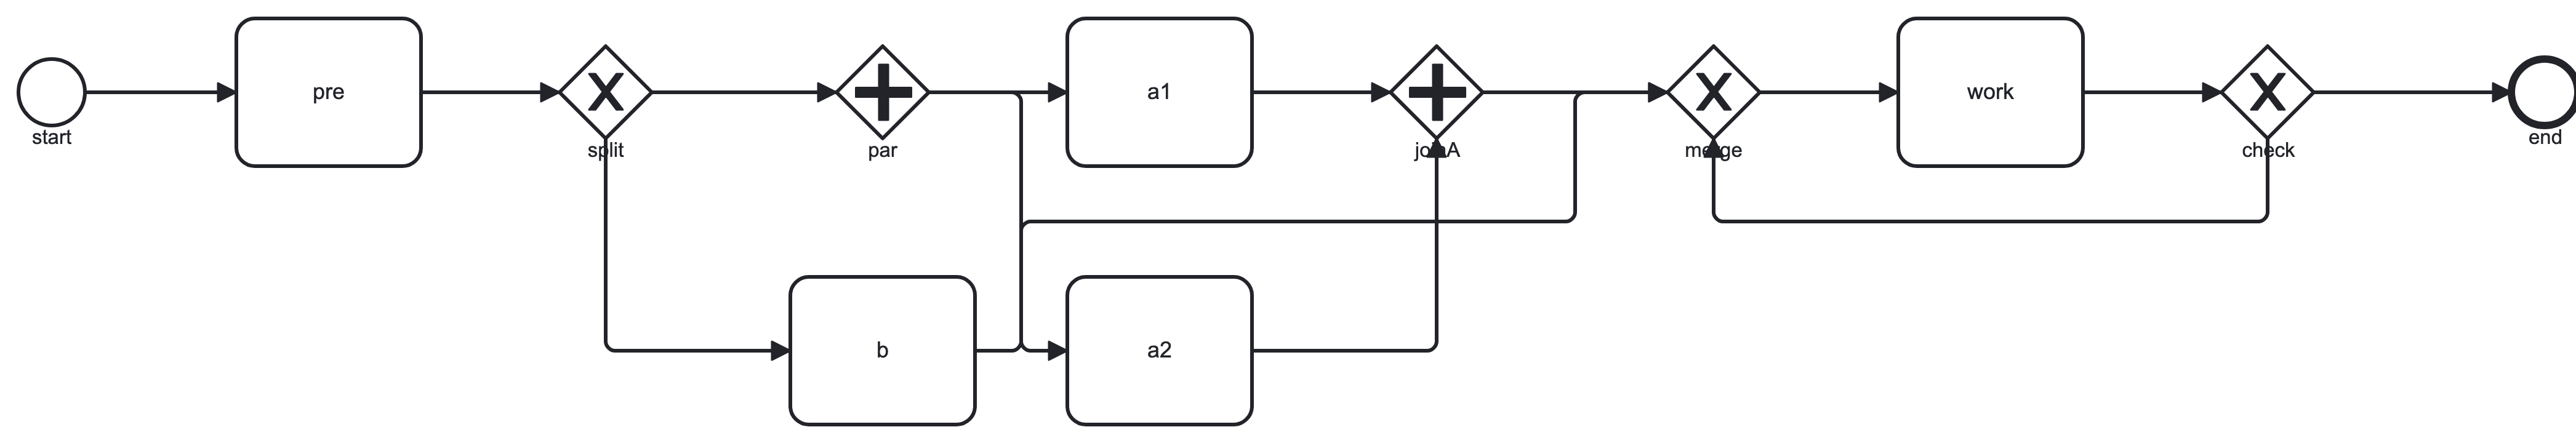
\includegraphics[width=\linewidth]{figures/models/composite}\\(g) choice + parallel pair + rework loop (V4)\end{minipage}
\caption{Generated BPMN test models used in the experiments; sources in \texttt{models/}.}
\label{fig:models}
\end{figure}

\begin{figure}[H]
\centering
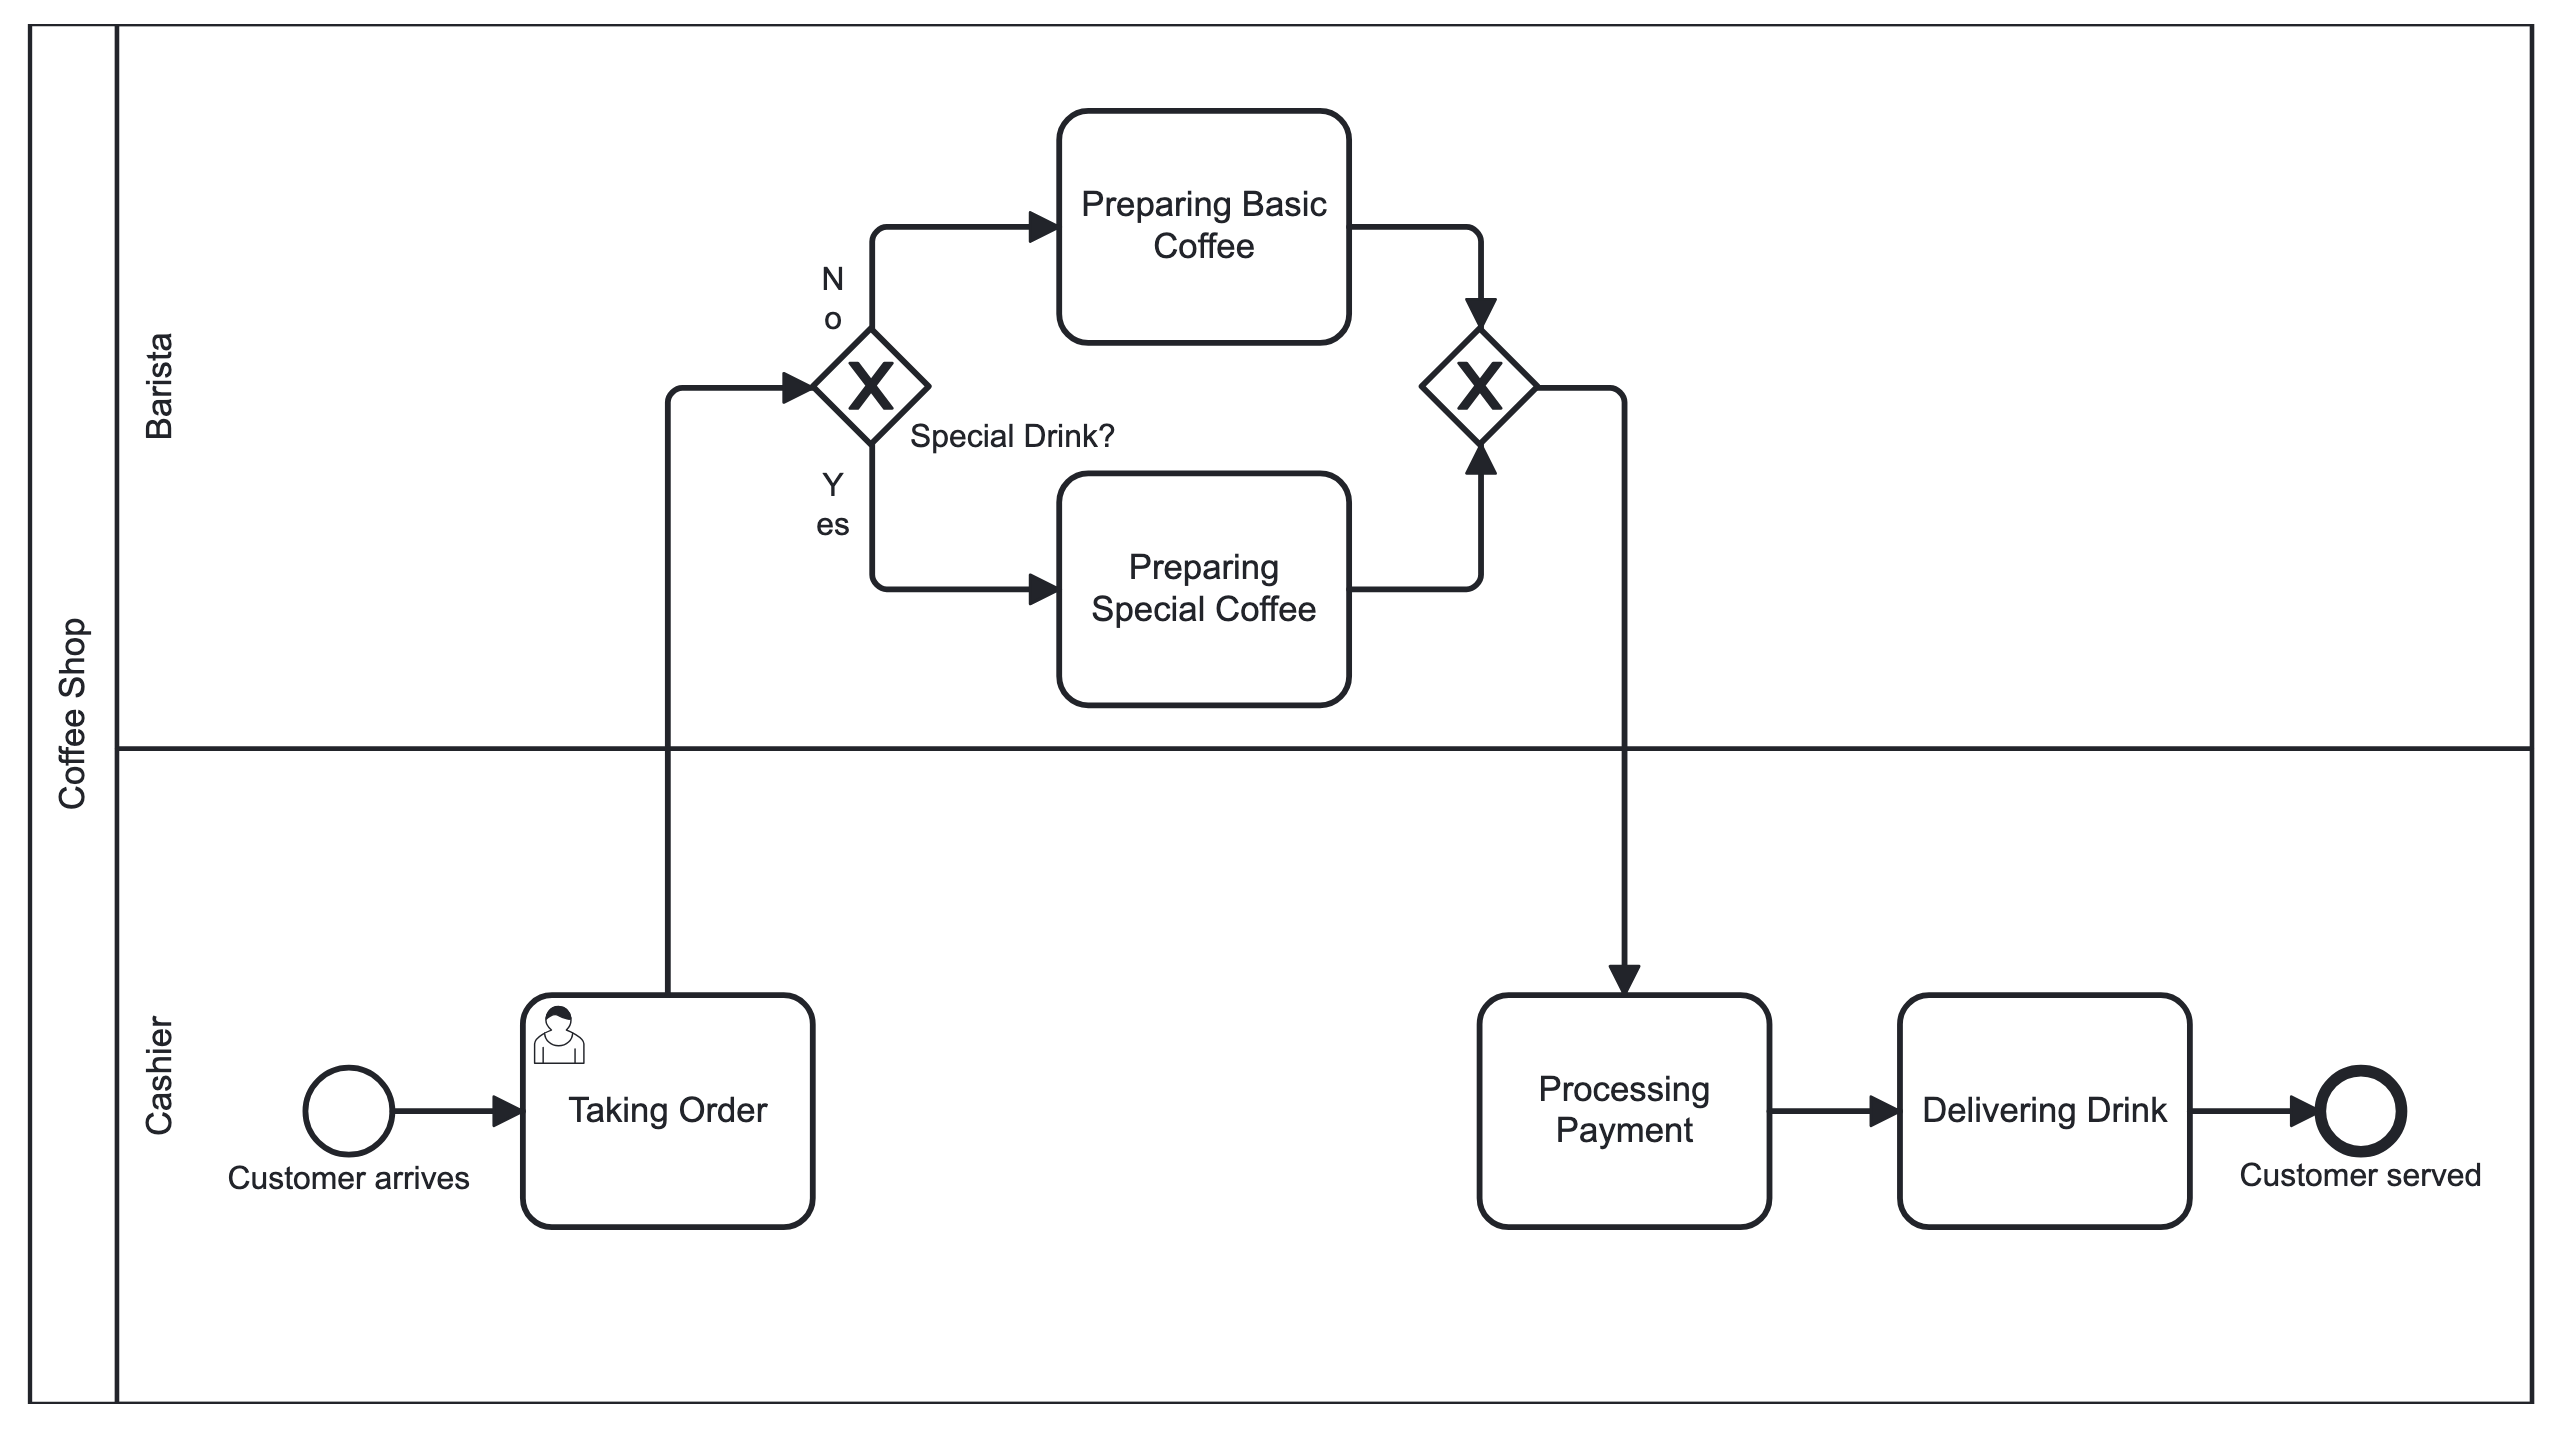
\includegraphics[width=\linewidth]{figures/models/coffee-shop}
\caption{The coffee-shop example shipped with the tool, used in the Prosimos cross-check (V2) and the decision experiment (V5).}
\label{fig:coffeemodel}
\end{figure}

\end{document}
